%%%% kr-instructions.tex -- version 1.3 (11-Jan-2021)

\typeout{KR2023 Instructions for Authors}

% These are the instructions for authors for KR-23.

\documentclass{article}
\pdfpagewidth=8.5in
\pdfpageheight=11in

\usepackage{kr}

% Use the postscript times font!
\usepackage{times}
\usepackage{soul}
\usepackage{url}
\usepackage[hidelinks]{hyperref}
\usepackage[utf8]{inputenc}
\usepackage[small]{caption}
\usepackage{graphicx}
\usepackage{amsmath}
\usepackage{amsthm}
\usepackage{amssymb}
\usepackage{booktabs}
\usepackage{algorithm}
%\usepackage{algorithmic}
\usepackage{xcolor}
\usepackage[noend]{algpseudocode}
\urlstyle{same}
\usepackage[inline]{enumitem}
\usepackage{subfig}
\usepackage{cleveref}

\usepackage{newfloat}
\usepackage{listings}
\DeclareCaptionStyle{ruled}{labelfont=normalfont,labelsep=colon,strut=off} % DO NOT CHANGE THIS
\lstset{%
	basicstyle={\normalsize\ttfamily},% footnotesize acceptable for monospace
	%numbers=left,numberstyle=\footnotesize,xleftmargin=2em,% show line numbers, remove this entire line if you don't want the numbers.
	aboveskip=0pt,belowskip=0pt,%
	showstringspaces=false,tabsize=2,breaklines=true,
	keywordstyle=\color{red},
	keywords={virginica,versicolor,setosa}}
\floatstyle{ruled}
\newfloat{listing}{tb}{lst}{}
\floatname{listing}{Listing}

\newcommand{\citet}[1]{\citeauthor{#1}~(\citeyear{#1})}
\newcommand{\citenop}[1]{\citeauthor{#1}~\citeyear{#1}}
\newcommand{\continue}{\textbf{continue}}
\newcommand{\undefined}{\textbf{undefined}}
\newcommand{\New}[1]{\textbf{new} #1}
\newcommand{\funskip}{\smallskip}
%\newcommand{\Comment}[1]{$\triangleright$ #1}
\DeclareMathOperator*{\argmin}{arg\,min}
\DeclareMathOperator*{\argmax}{arg\,max}
\DeclareMathOperator*{\avg}{avg}
\DeclareMathOperator*{\union}{\bigcup}

\newcommand{\xai}{XAI}
\newcommand{\psyke}{\textsc{PSyKE}}
\newcommand{\real}{\textsc{REAL}}
\newcommand{\trepan}{\textsc{Trepan}}
\newcommand{\iter}{\textsc{Iter}}
\newcommand{\gridex}{GridEx}
\newcommand{\gridrex}{GridREx}
\newcommand{\cream}{\textsc{CREAM}}
\newcommand{\creepy}{\textsc{CReEPy}}
\newcommand{\crash}{\textsc{CRASH}}
\newcommand{\pedro}{\textsc{PEDRO}}
\newcommand{\cart}{\textsc{Cart}}
\renewcommand{\smile}{Smile}
\newcommand{\scikit}{Scikit-Learn}
\newcommand{\exact}{ExACT}
\newcommand{\fire}{FiRe}
\newcommand{\psifire}{$\psi$-\fire}

%\newcommand\twoinarow{0.49\linewidth}
%\newcommand\twoinarowlarge{0.51\linewidth}
\newcommand\threeinarow{.3375\linewidth}
\newcommand\fourinarow{0.245\linewidth}

\newenvironment{inlinelist}{\begin{enumerate*}[label=\emph{(\roman{*})}]}{\end{enumerate*}}

% the following package is optional:
%\usepackage{latexsym}

% See https://www.overleaf.com/learn/latex/theorems_and_proofs
% for a nice explanation of how to define new theorems, but keep
% in mind that the amsthm package is already included in this
% template and that you must *not* alter the styling.
\newtheorem{example}{Example}
\newtheorem{theorem}{Theorem}

% Following comment is from ijcai97-submit.tex:
% The preparation of these files was supported by Schlumberger Palo Alto
% Research, AT\&T Bell Laboratories, and Morgan Kaufmann Publishers.
% Shirley Jowell, of Morgan Kaufmann Publishers, and Peter F.
% Patel-Schneider, of AT\&T Bell Laboratories collaborated on their
% preparation.

% These instructions can be modified and used in other conferences as long
% as credit to the authors and supporting agencies is retained, this notice
% is not changed, and further modification or reuse is not restricted.
% Neither Shirley Jowell nor Peter F. Patel-Schneider can be listed as
% contacts for providing assistance without their prior permission.

% To use for other conferences, change references to files and the
% conference appropriate and use other authors, contacts, publishers, and
% organizations.
% Also change the deadline and address for returning papers and the length and
% page charge instructions.
% Put where the files are available in the appropriate places.
%PDF Info Is REQUIRED.
\pdfinfo{
	/TemplateVersion (KR.2022.0, KR.2023.0)
}

%ricordarsi di cambiare la ref per creepy e di aggiungere quelle per psyke
\title{Symbolic Knowledge-Extraction Evaluation Metrics: The \fire{} Score}

% Multiple author syntax
\author{%
	Federico Sabbatini$^1$\and
	Roberta Calegari$^2$\\
	\affiliations
	$^1$Department of Pure and Applied Sciences (DiSPeA),\\University of Urbino\\
	$^2$Alma AI -- Alma Mater Research Institute for Human-Centered Artificial Intelligence,\\University of Bologna\\
	\emails
	f.sabbatini1@campus.uniurb.it,
	roberta.calegari@unibo.it
}

\begin{document}
	
\maketitle

\begin{abstract}
	Symbolic knowledge-extraction (SKE) techniques are becoming of key importance for AI applications since they enable the explanation of opaque black-box predictors, enhancing trust and transparency.
	%
	Among all the available SKE techniques, the best option for the case at hand should be selected.
	%
	However, an automatic comparison between different options can be performed only if an adequate metric -- such as a scoring function resuming all the interesting features of the extractors -- is provided. 
	%
	The definition of evaluation metrics for symbolic knowledge extractors is currently neglected in the literature.
	%
	Accordingly, in this paper we introduce the \fire{} score metric to assess the quality of a symbolic knowledge-extraction procedure, taking into account both its predictive performance and the readability of the extracted knowledge.
	%
	It is compared to another existing scoring metric and a rigorous mathematical formulation is provided along with several practical examples to highlight its effectiveness to the end of being exploited inside automatic hyper-parameter tuning procedures.
\end{abstract}

%%%%%%%%%%%%%%%%%%%%%%%
\section{Introduction}
%%%%%%%%%%%%%%%%%%%%%%%
One of the main strengths of machine learning (ML) models is their ability to provide exceptionally accurate predictions when applied in (roughly) every conceivable scenario~\cite{rocha2012far}.
%
Unfortunately, the most powerful ML predictors -- such as deep neural networks, for instance -- present a high price in terms of human interpretability of their outputs.
%
Indeed, they acquire knowledge during a training phase and store it in a sub-symbolic way, in the form of internal parameters.
%
This common \emph{opaque} behaviour constitutes a real barrier to the exploitation of such models, named \emph{black boxes} (BBs), in critical areas, that are all those real-world applications heavily impacting human lives, e.g., in terms of safety, health, and finance.

Different solutions have been proposed by the explainable artificial intelligence community to combine human interpretability with the predictive performance of BB models~\cite{guidotti2018survey}.
%
Amongst the strategies available in the literature there is the choice of intrinsic explainable models~\cite{Rudin2019}, such as decision trees with a limited amount of internal nodes and leaves.
%
When this option is not feasible or does not provide satisfying results, a different research branch suggests extracting the BB acquired knowledge by adhering to some \emph{symbolic} representation, through a reverse-engineering of the BB behaviour~\cite{KENNY2021103459}.
%
This second strategy is the rationale behind symbolic knowledge-extraction (SKE) procedures.

In the years, a plethora of SKE techniques has been proposed in the literature~\cite[for instance]{breiman1984classification,craven1994using,Thrun94,Andrews95rulex,craven1996extracting,BenitezCR97,SetionoL97,schmitz1999ann,SetionoL00,CastilloGP01,saito2002extracting,setiono2002extraction,Markowska-KaczmarT03,SetionoT04,barakat2005eclectic,huysmans2006iter,grex-icdm2008,NunezAC08,gridex-extraamas2021,gridrex-kr2022}.% and applied to several learning tasks \cite[to cite some examples]{bologna1997three,hayashi2000comparison,baesens2003using,hofmann2003rule,steiner2006using,franco2007early,sabbatini22LPFSKE}.
%
Given the amount of available analogous algorithms applicable to the same tasks, it may be complex to find the most suitable.
%
Furthermore, some procedures need the fine tuning of a set of hyper-parameters, usually requiring time and skills to be performed by users.

Comparisons between different instances of the same extractor, or different extractors, are usually carried out by observing
%
\begin{inlinelist}
	\item the predictive performance of the extractor, w.r.t.\ the underlying BB predictions and/or the actual data set output variables;
	\item the readability of the output human-intelligible knowledge; and
	\item the completeness of the knowledge in providing predictions~\cite{garcez2001symbolic,tran2013knowledge,skemetrics-aaai2023}.
\end{inlinelist}

The former can be easily assessed via the same metrics adopted to measure the predictive performance of the underlying BB (e.g., F$_1$ and accuracy scores for classification tasks and mean absolute/squared error and R$^2$ score for regression tasks).
%
Readability may be measured through different indicators, however, to the best of our knowledge, a widely-acknowledged, well-founded, and sound definition has not been yet formulated.
%
Finally, knowledge completeness may be calculated as the percentage of queries that the knowledge is able to predict.

Comparisons performed by users and automated algorithmic comparisons can surely benefit from a unified scoring function encompassing the concepts of predictive performance, readability and completeness associated with the knowledge provided by SKE techniques.
%
The definition of this kind of scoring is the fundamental brick for moving toward automated machine learning (AutoML) \cite{karmaker2021automl}.
%
Accordingly, in this paper we propose the \fire{} score as a compact and expressive metric to evaluate and compare different knowledge extractors, also in association with automated parameter tuning procedures.

The paper is organized as follows.
Section \ref{sec:motivation} discusses the motivations of the work as well as some considerations around the topic.
%
\Cref{sec:fire} contains the main contribution of this work and defines the \emph{\fire{} score} for the evaluation of symbolic knowledge.
\Cref{sec:use,sec:experiments} discuss the use of the metric as well as some explanatory experiments, respectively.

%%%%%%%%%%%%%%%%%%%%%%%
\section{Motivations}\label{sec:motivation}
%%%%%%%%%%%%%%%%%%%%%%%

SKE techniques have been applied in a wide variety of areas~\cite[to cite some examples]{bologna1997three,hayashi2000comparison,baesens2003using,hofmann2003rule,steiner2006using,franco2007early,sabbatini22LPFSKE}.
%%
%The process of knowledge extraction from opaque ML models can follow different paradigms, i.e., SKE algorithms can be either decompositional or pedagogical~\cite{andrews1995survey}.
%%
%In both cases, the output knowledge is generally represented as a set of logic rules, sometimes translated into natural language.
%%
%Decompositional techniques take into account the internal structure of the BB, that in turn is related to the BB nature.
%%
%For instance, decompositional algorithms suitable for artificial neural networks cannot be applied to support-vector machines.
%%
%Pedagogical techniques, on the other hand, are more general, since they are applicable to any kind of opaque model.
%%
%They only consider the output response corresponding to a given input instance or set of instances, with the aim of creating a mimicking, human-interpretable model able to approximate the underlying model predictions in the most adherent way.
%
Comparisons between different instances of the same extractor, or different extractors, in order to select the ``best extracted knowledge'' are usually carried out by observing the extractor's predictive performance, its completeness and the corresponding readability in terms of number of rules, by considering high values of these indices as more desirable.
%
Such a comparison in the literature is always done manually and just by looking at the three indices separately.
%
The comparison is therefore subjective: if knowledge $K_a$ is compared with another knowledge $K_b$ having the same readability and completeness but a smaller degree of predictive accuracy, then it is trivial to consider $K_a$ as the best one.
%
Conversely, if $K_a$ has the same completeness and predictive accuracy as $K_b$, but with a smaller readability extent, then the best knowledge is $K_b$.
%
It is also trivial to select the best knowledge if $K_a$ has at the same time all three indices with smaller values than knowledge $K_b$, which in this case would result as the best.
%
The main challenge is to decide which is the best output amongst all those provided by SKE techniques when there is no knowledge minimising the three indices contemporaneously.
%
It is always possible to highlight more than one optimum output, i.e., one for each evaluating criterion, but comparisons between small predictive performance increases versus small human-readability losses are subject to the human judgement and thus the identification of a single, optimum knowledge may depend on a subjective, biased selection.

We believe that the formulation of a standardised, compact scoring function encompassing multiple indices may lead to a more impartial knowledge quality assessment than the human comparison performed separately for each available evaluating criterion.
%
On the other hand, from an auto-ML perspective, only by enclosing multiple indices within a unique metric it is possible to design and implement hyper-parameter tuning algorithms for SKE techniques without neglecting relevant evaluating criteria.
%
For instance, a metric for knowledge quality evaluation may be a precious tool for giving robustness to the \pedro{} procedure~\cite{gridrex-kr2022}, a tool to automatically find the best parameter values for the \gridex{} and \gridrex{}~\cite{gridex-extraamas2021,gridrex-kr2022} knowledge-extraction algorithms.

To the best of our knowledge, not only an automatic way of evaluation is missing in the literature, but it is also missing a formal definition of metrics synergically combining predictive performance and readability to measure the quality of the extracted knowledge as a unique indicator, with the only exception proposed by~\citet{skemetrics-aaai2023}, where a scoring function involving predictive performance, readability and also completeness is presented.
%
The authors propose a multiplicative metric having three terms related to the indices.
%
More in detail, indices are expressed in terms of \emph{losses} (i.e., predictive loss, readability loss, and coverage loss) that should be as small as possible for good quality knowledge.
%
As a result, also the overall scoring function multiplying the three losses results small for good quality knowledge and therefore it is possible to assign scores to the extractors' outputs automatically and also to compare them within algorithmic parameter tuning routines.

The predictive performance of the extracted knowledge may be assessed w.r.t.\ two different dimensions by using the same scoring function adopted for the underlying BB.
%
These dimensions are:
%
\begin{inlinelist}
	\item the mimicking capabilities w.r.t.\ the underlying model predictions, usually called \emph{fidelity}; and
	\item the \emph{predictive performance} w.r.t.\ the data set output features.
\end{inlinelist}

Straightforward measurements of coverage and coverage loss are the rates of provided and missed predictions, respectively, w.r.t.\ the total amount of instances for which the knowledge has been queried.
%
Alternatively, it is possible to calculate the percentage of covered and uncovered regions of the input feature space, respectively.
%
Coverage is trivially equal to 1.0 for exhaustive knowledge-extraction algorithms, for instance, those based on decision trees.

The readability evaluation from a human perspective is usually done by comparing the number of extracted items (i.e., an algorithm that extracts 5 rules is considered more readable than an algorithm that extracts 10 rules; or an algorithm that extracts a decision tree with depth = 5 is considered more readable than an algorithm extracting a decision tree with depth = 10)~\cite{czarnowski2016}.
% 
Evaluation exclusively taking into account this level can be considered rather superficial since a wider set of indicators should be taken into account for a complete evaluation \cite{sabbatini2022-metrics}.
%
In particular, a readability metric may also consider:
%
\begin{inlinelist}
	\item the shape of the extracted knowledge, e.g., list or trees of rules, decision tables, etc.; and
	\item the readability of single atoms composing the knowledge, e.g., how individual rules or tree nodes and leaves are constructed.
\end{inlinelist}
%
However, both these items require further investigations to be formalised and numerically assessed.

The scoring function presented here considers only the knowledge size as readability measure, similar to comparisons performed by humans and reported in the literature.
%
The same strategy has been applied for the other metric described by~\citet{skemetrics-aaai2023}.

\fire{} differs from the existing metric for two reasons.
%
First, \fire{} neglects the contribution of the coverage index in calculating the overall score.
%
Thus, it is based only on the notions of predictive and readability losses.
%
Second, \fire{} allows users to provide an input parameter used to weight the contribution of the predictive loss w.r.t.\ the readability loss.
%
This is important, since it enhances the flexibility of the scoring function in capturing the needs of users, for instance preferring output knowledge with the smallest predictive error rather than the most readable knowledge having larger errors.

%%-----------------------------------------------------------%
%\subsection{On the knowledge readability: considerations and examples}\label{ssec:consideration}
%%-----------------------------------------------------------%
%As mentioned above, knowledge extracted from a BB via SKE comes in the form of lists, decision trees, or decision tables \cite{guidotti2018survey,huysmans2011empirical}. 
%%
%In the following, some considerations and examples of different levels of readability of these outputs are discussed, to make the reader understand all the features that a readability evaluation metric should take into account when formulated.
%
%It is worth noting that according to~\citeauthor{sabbatini2022-metrics}~(\citeyear{sabbatini2022-metrics}) rule lists and trees are equivalent, since starting from a tree it is possible to build a list of rules by converting each path from the tree root to a different leaf into a distinct rule.
%%
%Analogously, decision tables usually represent a rule per row (or column), so they can be easily translated into a list of rules. 
%%
%Hence, all the different output formats in terms of shape are traceable to each other to be compared fairly.
%
%There exist remarkable differences, however, between \emph{ordered} and \emph{unordered} lists, since in the first case rules are evaluated from the top to the bottom and, for this reason, bottom rules may be simplified by assuming as trivially false the conditions represented in the top rules.
%%
%This leads to more concise knowledge representations, but at the cost of human readability, since to interpret the output of the bottommost rule it is necessary to acknowledge as false all the others.
%%
%As a consequence, it is evident how the mere amount of output rules is a rough but reliable indicator of readability, but the readability of single rules presents tricky challenges that should be carefully investigated.
%
%Furthermore, rules (that come usually in form of logic rules) are usually implications having a set of preconditions (e.g., describing an input feature space subregion) and a postcondition (i.e., the output associated with inputs belonging to the subregion).
%%
%Preconditions and postconditions present different degrees of intrinsic readability.
%%
%In particular, examples of preconditions are {con\-junc\-tions}/disjunctions of \emph{if-then}, \emph{M-of-N}, oblique or fuzzy rules, in positive or negative form.
%%
%Also in this case the more compact representations are denoted by a smaller human readability and it is a difficult task to assign a numerical readability score to them.
%%
%For instance, a trivial count of conditions and/or constants and/or variables contained in the rules is not suitable to assess readability, and this is easily demonstrated by considering the following example.
%%
%A precondition expressed as
%%
%\begin{equation*}
%	if (X \geq 0.5) \wedge (X \leq 0.75)
%\end{equation*}
%%
%contains one variable, two conditions, and two constants.
%%
%An equivalent fuzzy rule in the form 
%%
%\begin{equation*}
%	if~X~is~medium
%\end{equation*}
%%
%has one variable as well, but only one condition and one constant.
%%
%However, it presents the same degree of readability for humans, that need to know the semantics of $medium$.
%%
%Finally, the same concept may be modelled as 
%%
%\begin{equation*}
%	if~X \in [0.5, 0.75],
%\end{equation*}
%%
%differing from the first representation in the number of conditions (1 vs. 2).
%%
%But, actually, the readability extent is absolutely equivalent.
%
%On the other hand, as a final consideration, postconditions may be constant values or some kind of function involving input features.
%%
%In the latter case, readability is obviously reduced.
%
%These basic examples show how quantitatively measuring the readability of ``extracted knowledge" is not so trivial, and also leads to non-quantitative and subjective parameters to be taken into consideration. For this reason, in this work, we will limit the metric to take into account only the number of rules as an index of human interpretability---which is, in any case, what is reflected in the literature today.

%%%%%%%%%%%%%%%%%%%%%%%
\section{The \fire{} score}\label{sec:fire}
%%%%%%%%%%%%%%%%%%%%%%%

\captionsetup[subfigure]{width=.4\linewidth}
\begin{figure}[tb]\centering
	\subfloat[1-\fire{}.]{
		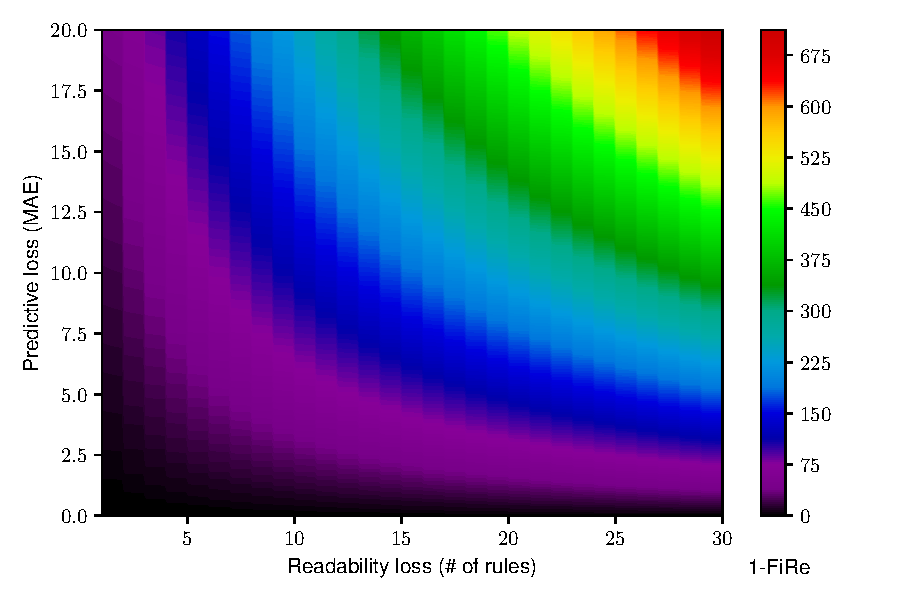
\includegraphics[width=0.5\linewidth]{figures/psi_1_color.pdf}\label{fig:psi1}
	}
	\subfloat[3-\fire{}.]{
		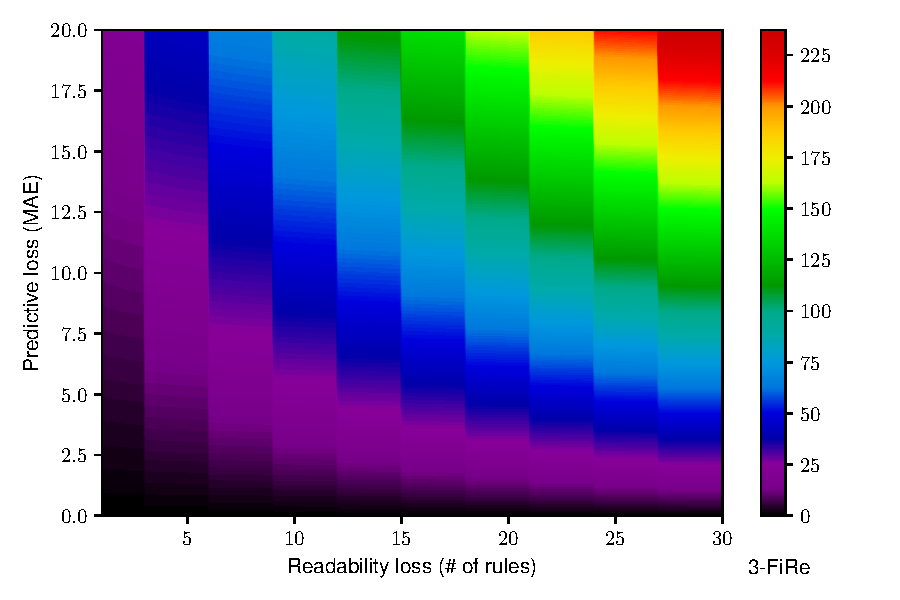
\includegraphics[width=0.5\linewidth]{figures/psi_3_color.pdf}\label{fig:psi3}
	}
	\\
	\subfloat[5-\fire{}.]{
		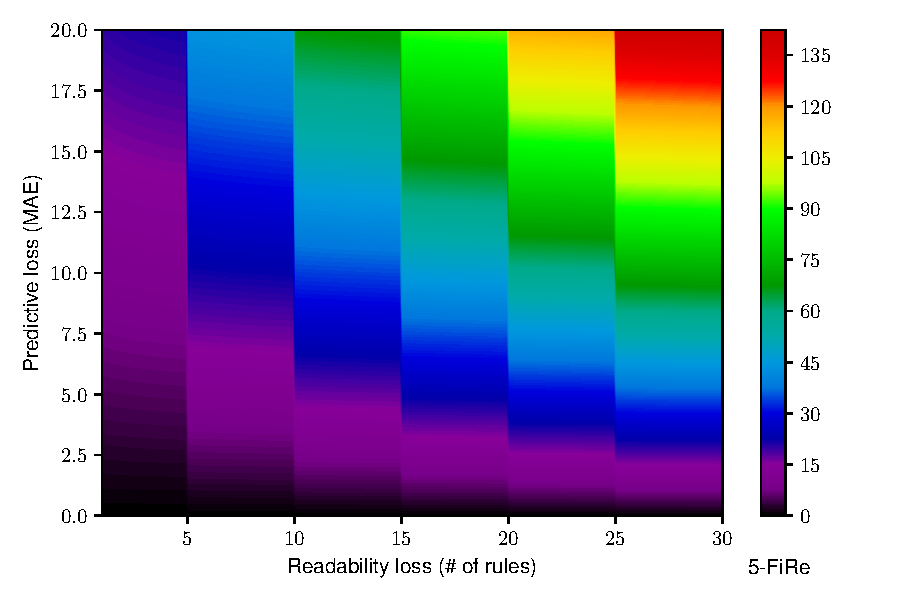
\includegraphics[width=0.5\linewidth]{figures/psi_5_color.pdf}\label{fig:psi5}
	}
	\subfloat[10-\fire{}.]{
		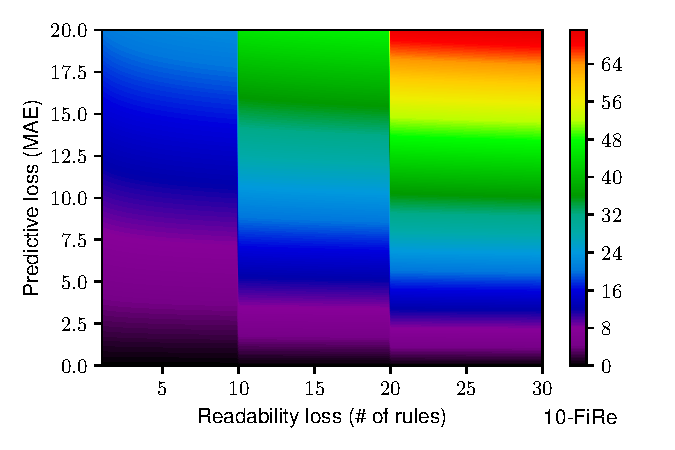
\includegraphics[width=0.5\linewidth]{figures/psi_10_color.pdf}\label{fig:psi10}
	}
	\caption{Graphs of different \psifire{} scoring functions, having $\psi \in \{1, 3, 5, 10\}$.}\label{fig:psi}
\end{figure}

The \fire{} scoring metric formulated for measuring the quality of the knowledge extracted via SKE considers both the knowledge's predictive performance and its readability, intended as human interpretability w.r.t.\ the amount of extracted rules.
%
The \fire{} score is thus a multivariate function defined as follows:
%
\begin{align}
	&\fire: \left( \mathbb{R}_{>0} \times \mathbb{R}_{\geq 0} \times \mathbb{R}_{\geq1} \right) \mapsto \mathbb{R}_{\geq 0},\\
	&\fire(\psi, p, r) = p \left \lceil{\frac{r}{\psi}}\right \rceil r^{0.05},
\end{align}
%
where $\psi$ is the fidelity/readability trade-off extent, $p$ is a measure of the predictive loss of the extractor and $r$ is a measure of its readability loss.

%-----------------------------------------------------%
\subsection{Variables and parameters}\label{sec:fire-var}
%-----------------------------------------------------%
As for the predictive loss $p$, a good measure in regression tasks is the mean absolute error (MAE) of the extractor's predictions w.r.t.\ the underlying BB predictions or the data set outputs, depending on the need.
%
For classification tasks, it is possible to use metrics anti-correlated with the accuracy score, e.g., $1-accuracy$.
%
The presented \fire{} score adopts the mean absolute error metric for regression, but it may be substituted with the mean squared error without substantial differences since both of them are generally correlated.
%
Analogously, metrics inversely proportional to the R$^2$ value may be also exploited.

As for the readability loss $r$, the total amount of output rules is a suitable metric and thus it is the one adopted to calculate the \fire{} score.
%
More complex options will be evaluated in the future, e.g., by taking into account the complexity of individual rules.

Finally, the $\psi$ parameter -- the only user-defined parameter -- describes how much the predictive loss can be penalised w.r.t.\ the readability loss.
%
It is important because, depending on the task at hand, the two losses may have different weights.
%
In particular, $\psi=1$ assigns the same importance to both losses.
%
Growing $\psi$ values tend to neglect the readability loss impact.
%
In other words, given the aforementioned \fire{} score formulation and by assuming to have extracted $m$ rules, if users set $\psi=n$ the \fire{} score will consider only $\frac{m}{n}$ rules, rounded up to the nearest integer.

%-----------------------------------------------------%
\subsection{Function domain}\label{sec:fire-domain}
%-----------------------------------------------------%
The domain of the function is explained by the following observations.
%
The $\psi$ parameter is a positive real value for design.
%
Limiting the admissible $\psi$ values to $\mathbb{N}_1$ may be also reasonable, but an extension to $\mathbb{R}_{>0}$ makes the \fire{} score more flexible.
%
On the other hand, the $p$ parameter is a measurement of a predictive error, so it may be equal to 0 in the best case, or arbitrarily larger otherwise since there is no upper bound to the predictive error of a model.
%
Finally, $r$ is an integer number greater or equal to 1, since it represents the number of extracted rules, that is a discrete quantity equal to 1 (in the best case) or larger (otherwise).
%
However, the admissible values for this parameter have been extended from $\mathbb{N}_1$ to $\mathbb{R}_{\geq 1}$ for the sake of flexibility, analogously to the range for $\psi$.
%
This choice enables, for instance, the \fire{} score calculation for averaged sets of extractors trained with the same hyper-parameters, resulting in a more robust score.

As a result of the observations above, the \fire{} score is defined as a continuous (yet non-differentiable) function in the aforementioned domain and it may assume any non-negative value.
%
Therefore, the score is a function bounded from below by 0.

%-----------------------------------------------------%
\subsection{Score meaning}\label{sec:fire-meaning}
%-----------------------------------------------------%

In the following, we use the notation \psifire{}($p$, $r$) as a clearer alias of \fire{}($\psi$, $p$, $r$) and we consider without loss of generality the \psifire{}($\cdot$) function as a bivariate function, by assuming the $\psi$ parameter fixed \emph{a priori}.

\captionsetup[subfigure]{width=.45\linewidth}
\begin{figure}[tb]\centering
	\subfloat[Trend of 5-\fire{} w.r.t.\ readability loss for different predictive loss values.]{
		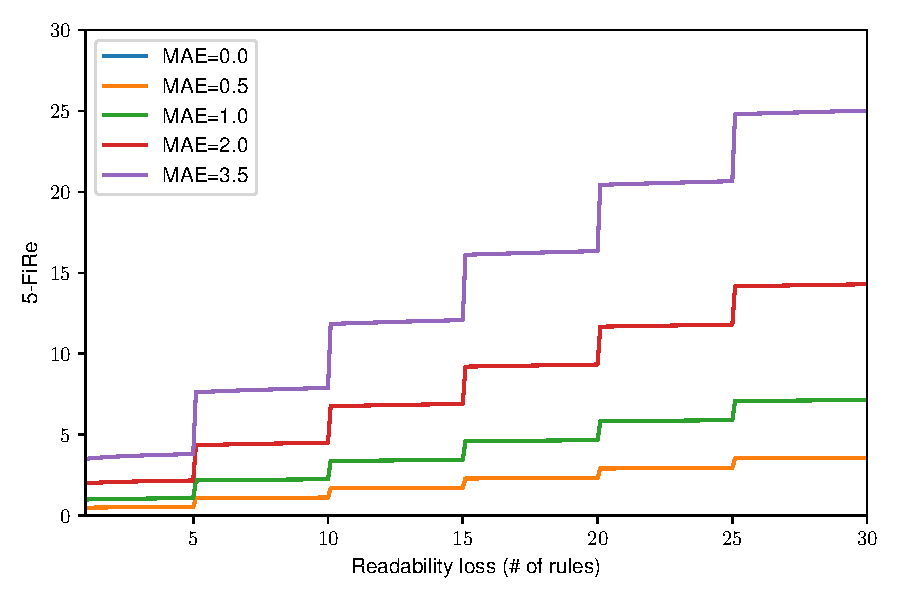
\includegraphics[width=0.5\linewidth]{figures/readVSfire.pdf}\label{fig:readVSfire}
	}
	\subfloat[Trends of several \psifire{} functions having equal predictive loss w.r.t.\ readability loss.]{
		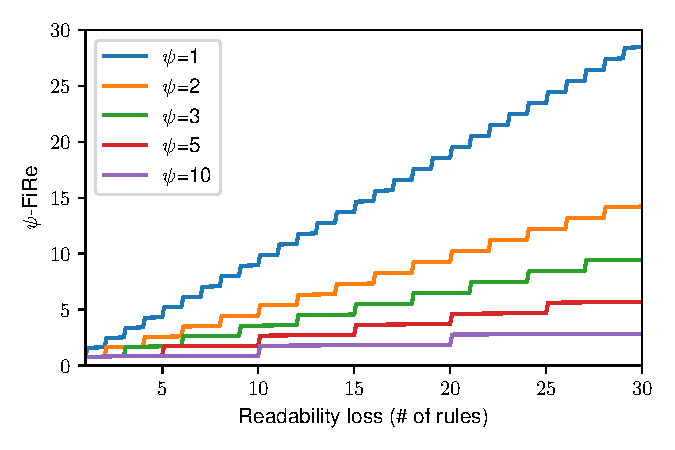
\includegraphics[width=0.5\linewidth]{figures/readVSfirePSI.pdf}\label{fig:readVSfirePSI}
	}
	\\
	\subfloat[Trend of 5-\fire{} w.r.t.\ predictive loss for different readability loss values.]{
		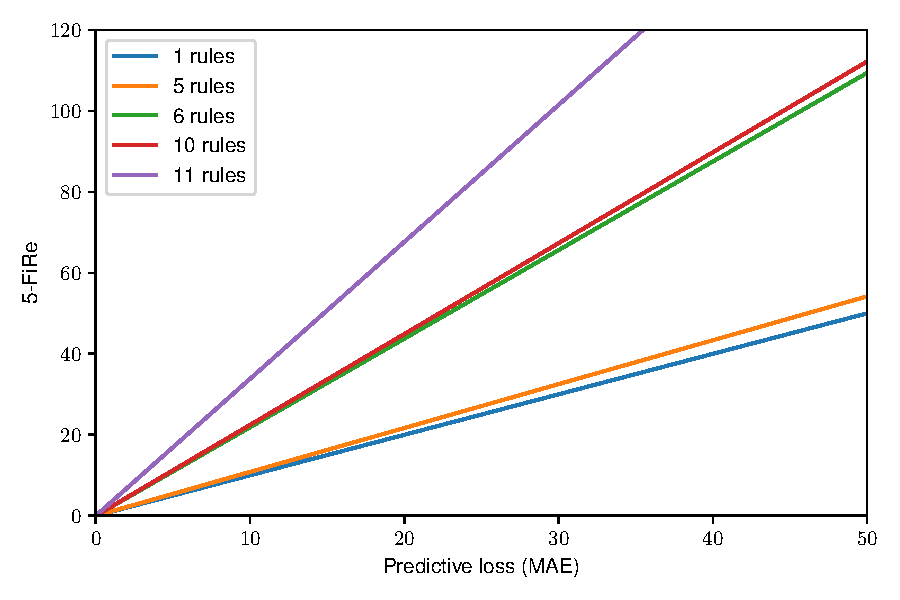
\includegraphics[width=0.5\linewidth]{figures/maeVSfire.pdf}\label{fig:maeVSfire}
	}
	\subfloat[Trends of several \psifire{} functions with equal readability loss w.r.t.\ predictive loss.]{
		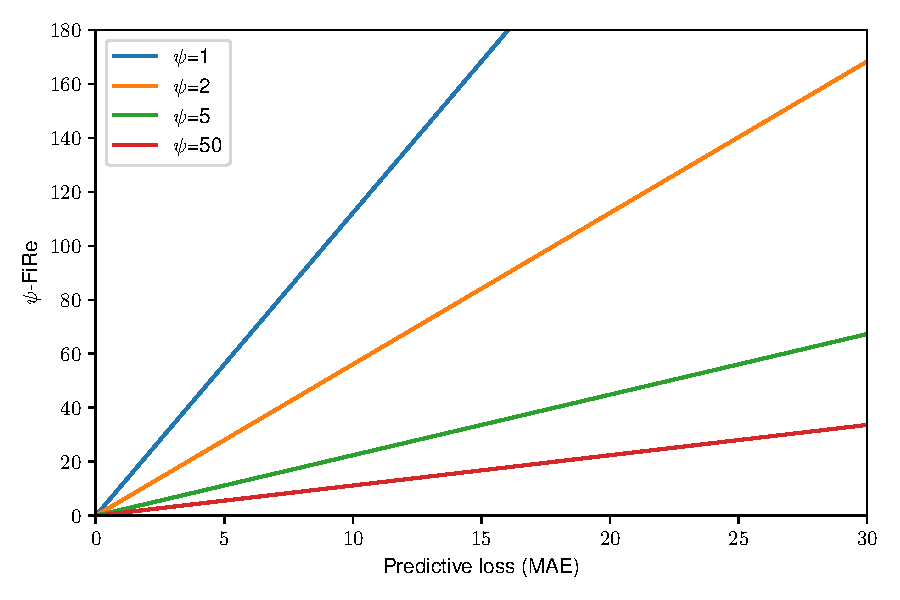
\includegraphics[width=0.5\linewidth]{figures/maeVSfirePSI.pdf}\label{fig:maeVSfirePSI}
	}
	\caption{Projections of several \psifire{} functions w.r.t.\ different values of $\psi$, readability loss and predictive loss.}\label{fig:proj}
\end{figure}

The \fire{} score has been formulated to assign low scores to desirable extractors.
%
It assumes that a good extractor should exhibit a low predictive loss and a low readability loss.
%
For this reason, it is a multiplicative score between the two parameters and, therefore, it is sufficient that only one amongst the predictive or the readability loss is high to bring the \fire{} score towards high values corresponding to low-quality knowledge.

The ceiling function appearing as the second factor of the score has the purpose to give a step-function shape to the \fire{} score.
%
The exact shape of the steps is regulated through the $\psi$ parameter, acting as a user-defined sensitivity threshold and thus appearing as the denominator in the second term of the score formulation.
%
By setting $\psi=n$, users impose these steps to have a length equal to $n$.
%
Since a flat step would assign the same \psifire{} score to extractors having the same predictive loss and a different but similar readability loss (e.g., $r$ = 1 and 2, respectively, and $\psi=10$), a third factor is queued to the score definition to discern amongst the extractors lying on the same step which one has to be considered the best.
%
We found that an exponent equal to 0.05 allows the scoring function to preserve all its peculiarities, at the same time adding the desired increasing trend to the step function (monotonicity).
%
In this way the \fire{} score keeps the step-function shape but becomes an increasing monotonic function (for any $p>0$, since $\psi\textrm{-}\fire{}(0, r)=0, \forall r, \forall \psi$).
%
We stress here that $p=0$ is a theoretically possible scenario, but it is practically impossible to obtain a model having no predictive error.
%
Examples of \psifire{} graphs are reported in \Cref{fig:psi}, for different values of $\psi$, $p$ and $r$.

%-----------------------------------------------------%
\subsection{Properties}\label{sec:fire-prop}
%-----------------------------------------------------%
The monotonicity of the \psifire{} score is ensured by the following conditions:
\begin{description}
	\item[monotonicity w.r.t.\ the projection of $p$] (cf.\ \Cref{fig:readVSfire})
	\begin{equation}
		\begin{split}
			r_1 < r_2 \iff &\psi\textrm{-}\fire(p, r_1) < \psi\textrm{-}\fire(p, r_2), \\ &\forall p \in \mathbb{R}_{>0}, ~~~\forall r_1, r_2 \in \mathbb{R}_{\geq1}
		\end{split}\label{eq:projP}
	\end{equation}
	\item[monotonicity w.r.t.\ the projection of $r$] (cf.\ \Cref{fig:maeVSfire})
	\begin{equation}
		\begin{split}
			p_1 < p_2 \iff &\psi\textrm{-}\fire(p_1, r) < \psi\textrm{-}\fire(p_2, r), \\ &\forall r \in \mathbb{R}_{\geq1}, ~~~\forall p_1, p_2 \in \mathbb{R}_{>0}
		\end{split}\label{eq:projR}
	\end{equation}
\end{description}
%
Alternatively, \Cref{eq:projP,eq:projR} can be substituted by the following condition:
%
\begin{description}
	\item[monotonicity w.r.t.\ a partial order on the domain] 
	\begin{equation}
		\begin{split}
			&(p_1 < p_2) \wedge (r_1 < r_2) \iff \\&\iff \psi\textrm{-}\fire(p_1, r_1) < \psi\textrm{-}\fire(p_2, r_2), \\ &\forall p_1, p_2 \in \mathbb{R}_{>0}, ~~~\forall r_1, r_2 \in \mathbb{R}_{\geq1}
		\end{split}\label{eq:partial}
	\end{equation}
\end{description}
%
\Cref{eq:projP,eq:projR,eq:partial} also hold by substituting $<$ with $>$.

The increasing trend of the score may be observed in \Cref{fig:proj} and it is demonstrated through its partial derivatives.
%
\Cref{eq:projP,eq:projR,eq:partial} hold for any possible $\psi>0$ that may be assigned to the \psifire{} score, as it is possible to notice from \Cref{fig:readVSfirePSI,fig:maeVSfirePSI}.

The partial derivative w.r.t.\ $p$ is the following:
%
\begin{equation}
	\frac{\partial \psi\textrm{-}\fire}{\partial p} = \left \lceil{\frac{r}{\psi}}\right \rceil r^{0.05} \label{eq:partialP}
\end{equation}
%
always positive and defined in the whole domain.
%
The partial derivative w.r.t.\ $r$ is the following:
%
\begin{equation}
	\frac{\partial \psi\textrm{-}\fire}{\partial r} = \frac{0.05 p \left \lceil{\frac{r}{\psi}}\right \rceil}{r^{0.95}}\label{eq:partialR}
\end{equation}
%
always positive for $p>0$ and defined in the whole domain except for $\frac{r}{\psi} \in \mathbb{Z}$.
%
The derivative is 0 for $p=0$, indeed in this case the \psifire{} score is always 0 regardless of the values of $\psi$ and $r$.

%%%%%%%%%%%%%%%%%%%%%%%
\section{On the practical use of \fire{}}\label{sec:use}
%%%%%%%%%%%%%%%%%%%%%%%

In this section considerations about the practical application of the \fire{} score are reported, in order to highlight its effectiveness but also to further explain the score meaning and the importance of the $\psi$ parameter.
%
Accordingly, in \Cref{ssec:comp} several examples of the \fire{} score applications are explained, together with corresponding observations, whereas in \Cref{ssec:balance} the equilibrium between the predictive and readability loss parameters is analytically studied. Finally, in \Cref{ssec:psi} more details about the $\psi$ parameter tuning are provided from a practical application standpoint.

\subsection{Comparing algorithms with \fire{}}\label{ssec:comp}

\begin{figure}
	\centering
	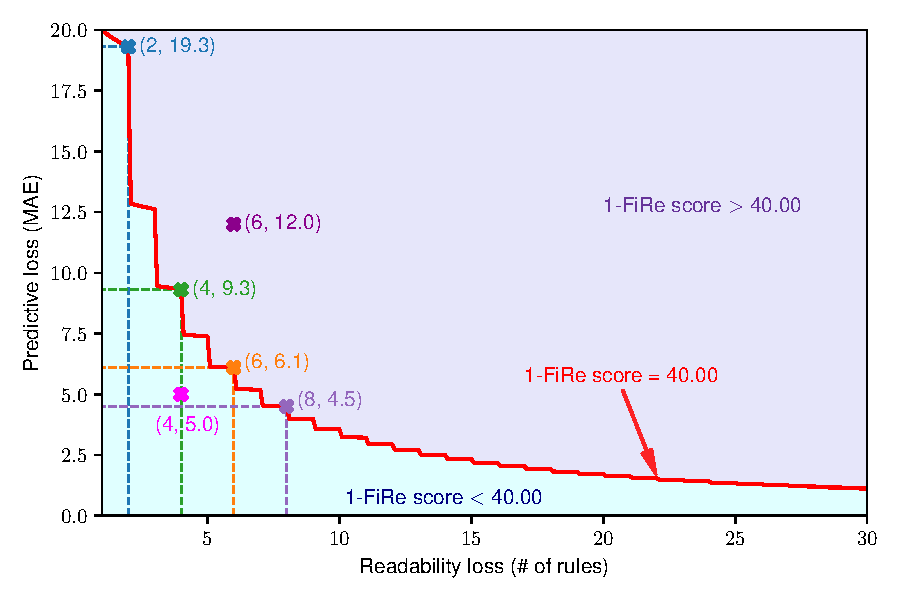
\includegraphics[width=\linewidth]{figures/boundaries.pdf}
	\caption{Graphical representation of the boundaries identified by the 1-\fire{} score (isoline for $1\textrm{-}\fire{}=40.0$).}\label{fig:boundaries}
\end{figure}

Given all the aforementioned properties about the \fire{} scoring function, we exemplify here some applicative scenarios from a theoretical point of view.
%
Let us assume to have an extraction procedure providing as output knowledge a single human-interpretable rule.
%
The mean absolute error associated with this rule is equal to 40.0 and we chose to adopt $\psi=1$.
%
As a consequence, $1\textrm{-}\fire(40.0, 1)=40.0$.

In \Cref{fig:boundaries} the isoline corresponding to a 1-\fire{} score equal to 40.0 is represented in red.
%
Readability loss and predictive loss are reported on the x-axis and y-axis, respectively, as the number of extracted rules and mean absolute error.
%
The extractor under study, with 1 rule and a predictive error equal to 40.0, lies on the red isoline.
%
The same condition holds for all extractors having the same 1-\fire{} score value.
%
This is the case, for example, of extractors providing 2, 4, 6 and 8 rules associated with MAE of 19.3, 9.3, 6.1 and 4.5, respectively.
%
All these models are considered \emph{equivalent} on the basis of the 1-\fire{} score.
%
Conversely, a model able to extract 4 rules with a predictive error of 5.0 is considered \emph{better}, since it has a smaller 1-\fire{} score and thus it lies in the graph under the red isoline.
%
More precisely, $1\textrm{-}\fire(5.0, 4)=21.4$.
%
On the other hand, an extractor providing 6 rules with MAE = 12.0 is considered \emph{worse}, since its 1-\fire{} score is greater than 40.0 and thus it graphically lies above the red isoline.
%
Indeed, $1\textrm{-}\fire(12.0, 6)=78.7$.
%
These two latter examples have the purpose of demonstrating that the \fire{} score is still effective even if only one amongst the predictive or readability losses is subject to changes.

\Cref{fig:boundaries} clearly highlights how the \fire{} score identifies an exact boundary separating, w.r.t.\ a given extractor, the sets of equivalent, worse and better extractors.
%
Furthermore, the isoline depicts the fidelity/readability trade-off correlated to $\psi=1$.
%
%Indeed, this is the smallest admissible value for the parameter, and it is the value assigning the maximum importance to readability losses.
%
By observing the red isoline it is noticeable how a doubling of the readability loss (e.g., from 2 to 4) is accepted only if it is approximately balanced with a halving of the predictive loss.
%
The curve can be also read in the opposite sense, e.g., a doubling of the predictive loss is accepted only when (approximately) compensated by a readability loss halving.
%
With this reading key, it is possible to exploit the \fire{} isolines to analytically study better and worse extraction procedures w.r.t.\ a fixed one, by taking into consideration both increases and decreases of the predictive loss and/or of the readability loss.

Finally, we exploit the same figure to stress the fact that the isoline presents an asymptotic trend when the $p$ and $r$ parameters tend to infinity.
%
This behaviour reflects the actual quality of the knowledge provided by SKE techniques.
%
Indeed, when the number of rules or the predictive error is very high, the evaluated knowledge has low quality and it is no more a relevant task to have a fine-grained measure of \emph{how} a loss should be compensated by the other.

\subsection{Predictive and readability loss equilibrium}\label{ssec:balance}

Given the ability of the \fire{} score in providing the notion of \emph{knowledge equivalence} according to more than one index, SKE techniques' users have the possibility to perform analytical investigations on the knowledge quality to understand
%
\begin{inlinelist}
	\item the predictive loss decrease (resp.\ increase) exactly annihilating a readability loss increase (resp.\ decrease); and
	\item the predictive loss decrease (resp.\ increase) having the same effect as a readability loss decrease (resp.\ increase).
\end{inlinelist}
%
This enables not only the knowledge evaluation and the best knowledge selection, but also a pairwise comparison based on predictive and readability loss alteration.

In the first case, the goal is to find the equilibrium between predictive loss and readability loss when both these indices vary in opposite directions (one increasing, leading to a worse \fire{} score and the other decreasing, leading to a better score).
%
This allows users to spot a set of equivalent knowledge and therefore to analytically observe the corresponding \fire{} isolines, understanding how to set the $\psi$ parameter.

In the second case, the focus is on studying the effects of individual decreases or increases in the losses to find equivalent pairs.
%
Thanks to this, users highlight the effect of the fidelity/readability $\psi$ trade-off and thus they may discover that it may be sufficient a small enhancement in one loss rather than big efforts on the other to achieve better knowledge quality.

In order to find the equilibrium between predictive and readability losses, the relationship to be satisfied can be expressed by the following equivalence, where $\alpha$ and $\beta$ are two unknown constants:
%
\begin{equation}\label{eq:equi1}
	\psi\textrm{-}\fire(p, r) = \psi\textrm{-}\fire(\alpha p, \beta r),
\end{equation}
%
that is equivalent to:
%
\begin{equation}\label{eq:equi2}
	p \left \lceil{\frac{r}{\psi}}\right \rceil r^{0.05} = \alpha p \left \lceil{\frac{\beta r}{\psi}}\right \rceil (\beta r)^{0.05}.
\end{equation}
%
By resolving w.r.t.\ $\alpha$ we obtain:
%
\begin{equation}\label{eq:alpha}
	\alpha = \frac{\left \lceil{\frac{r}{\psi}}\right \rceil}{\left \lceil{\frac{\beta r}{\psi}}\right \rceil \beta^{0.05}}.
\end{equation}

These equations demonstrate that knowledge with a predictive loss $p$ and readability loss $r$ has the same quality as another knowledge having predictive loss $\alpha p$ and readability loss $\beta r$ if and only if \Cref{eq:alpha} is satisfied.
%
Furthermore, \Cref{eq:alpha} highlights that the $p$ parameter is not relevant in finding a pair of compensating $\alpha$ and $\beta$ multiplicative constants for the losses involved in the \fire{} score calculation, differently to $r$ and $\psi$ that play a role in the pair determination.
%
This is not surprising, given that the \fire{} score is directly proportional to the predictive loss and therefore the increasing score (denoting a quality worsening) due to a predictive loss increase is not dependent on the actual value of the loss before or after the increase.
%
Conversely, how a readability loss increase affects the \fire{} score is strictly dependent on the loss value itself and the $\psi$ parameter.

When altering the predictive and readability losses in the \fire{} score, given the monotonicity properties of the scoring function, intuitively we may have predictive loss increases compensated by readability loss decreases or, vice versa, readability loss increases balanced by predictive loss decreases.
%
\Cref{eq:alpha} confirms this intuition.
%
Indeed, readability loss increases are represented with $\beta > 1$ values.
%
This implies that $\beta^{0.05} > 1$ and that $\left \lceil{\frac{r}{\psi}}\right \rceil \leq \left \lceil{\frac{\beta r}{\psi}}\right \rceil$.
%
Thus, if $\beta > 1$ then $\alpha < 1$.
%
Conversely, if $\beta < 1$ then $\beta^{0.05} < 1$ and $\left \lceil{\frac{r}{\psi}}\right \rceil \geq \left \lceil{\frac{\beta r}{\psi}}\right \rceil$.
%
Therefore, if $\beta < 1$ then $\alpha > 1$.
%
Obviously, if $\beta = 1$ then $\alpha = 1$.

All these relationships may be traced in \Cref{fig:equi}.
%
In the figure, the relationship between the $\alpha$ and $\beta$ values are shown for different values of the threshold-parameter $\psi$ and the readability loss $r$, given that $\alpha$ depends also on them other than $\beta$.
%
It is possible to notice that with a fixed $\beta$ and for growing values of $\psi$ the effects of $\beta$ are more and more neglected, whereas for growing values of $r$ they are more pronounced.
%
As a consequence, when $\beta > 1$ increasing $\psi$ or decreasing $r$ implies increasing $\alpha$.
%
Conversely, when $\beta < 1$ increasing $\psi$ as well as decreasing $r$ induces decreasing $\alpha$ values.

\begin{figure}
	\centering
	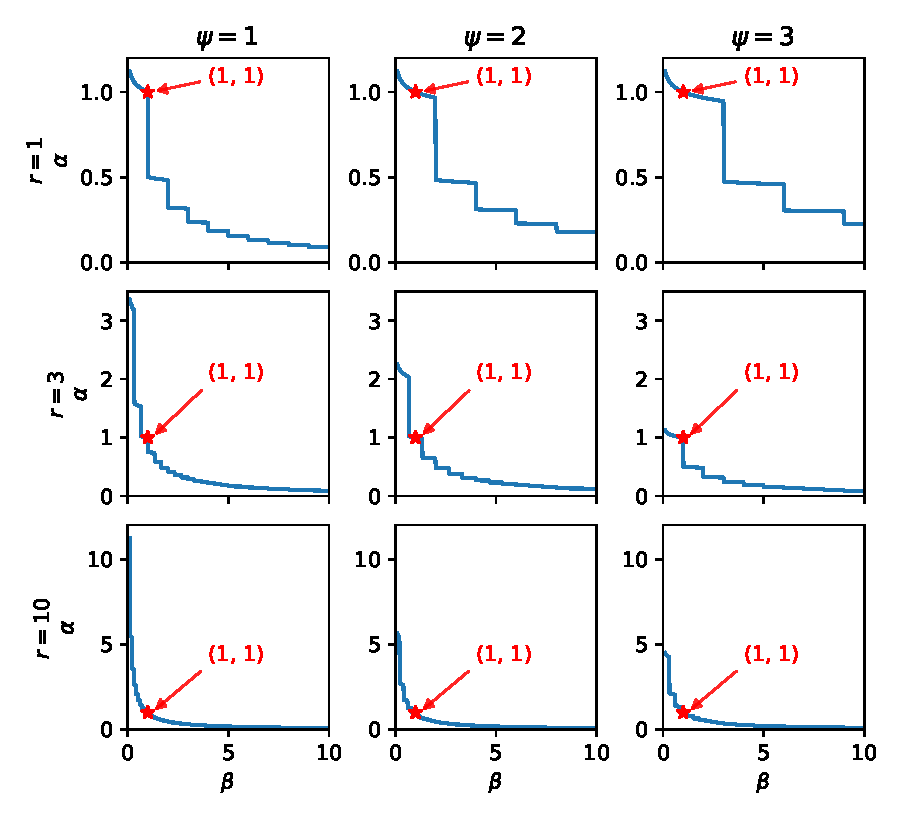
\includegraphics[width=1.02\linewidth]{figures/equi.pdf}
	\caption{Equilibrium between $\alpha$ and $\beta$ for different values of the readability loss $r$ and the $\psi$ parameter.}\label{fig:equi}
\end{figure}

To conclude the analysis of the entanglement between the predictive and readability losses, we point out that in order to find equivalent pairs of increases/decreases in the predictive and readability losses it is sufficient to modify \Cref{eq:equi1} as follows:
%
\begin{equation}\label{eq:equi3}
	\psi\textrm{-}\fire(\alpha p, r) = \psi\textrm{-}\fire(p, \beta r).
\end{equation}
%
Developing the equation similar to the equilibrium case we find:
%
\begin{equation}\label{eq:alpha2}
	\alpha = \frac{\left \lceil{\frac{\beta r}{\psi}}\right \rceil \beta^{0.05}}{\left \lceil{\frac{r}{\psi}}\right \rceil}.
\end{equation}
%
By applying the same considerations as before, we find that in this case $\alpha$ and $\beta$ are both $=1$, $<1$, or $>1$.

\subsection{Tuning the $\psi$ parameter}\label{ssec:psi}

\begin{figure}
	\centering
	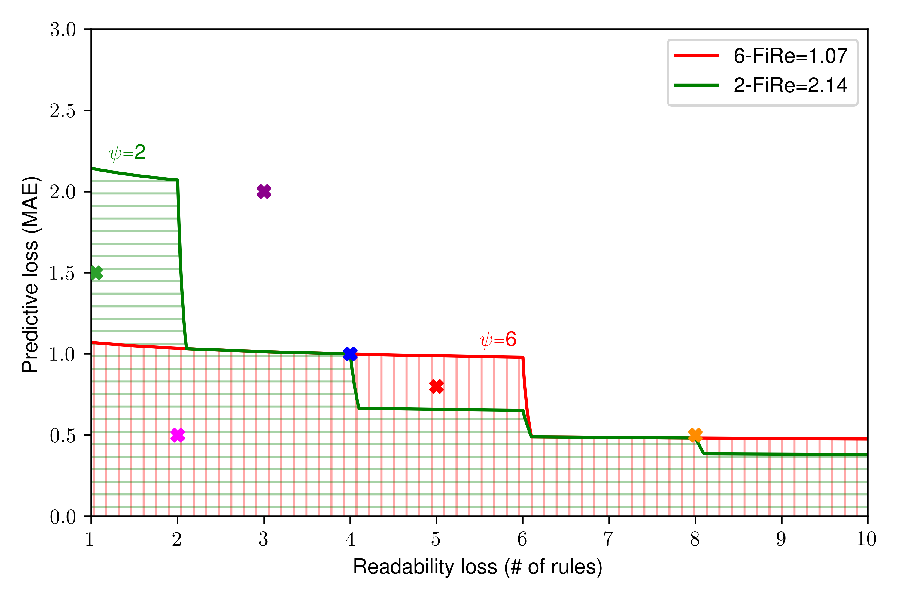
\includegraphics[width=\linewidth]{figures/areas.pdf}
	\caption{Different boundaries associated to the 2-\fire{} and 6-\fire{} scores.}\label{fig:areas}
\end{figure}

It is of fundamental importance to carefully choose the $\psi$ parameter of \fire{}.
%
\Cref{fig:readVSfirePSI} already showed that larger values of $\psi$ reduce the impact of the readability loss.
%
However, it is important to know that different $\psi$ values may lead to \emph{opposite} results when applied to compare the same extractors.
%
This peculiarity is depicted in \Cref{fig:areas}, representing the separating boundaries identified by the isolines obtained via the 2-\fire{} and 6-\fire{} scores w.r.t.\ a given extractor described in the following.
%
The boundaries associated with the two scoring functions are represented as green and red isolines, respectively.
%
The hatched area below each isoline highlights the parameter space region denoting ``more desirable'' extractors, providing knowledge with better quality w.r.t.\ extractors lying on the isoline.

Let us assume to have an extractor able to obtain 4 rules from a BB model with a mean absolute error equal to 1.0 (blue cross in \Cref{fig:areas}).
%
The \psifire{} scores associated with this model are:
%
\begin{equation*}
	2\textrm{-}\fire(1.0, 4)=2.14,
\end{equation*}
%
\begin{equation*}
	6\textrm{-}\fire(1.0, 4)=1.07.
\end{equation*}
%
An SKE algorithm extracting 8 rules with MAE = 0.5 (orange cross) has the same \fire{} scores for both values of $\psi$.
%
The models are thus equivalent according to both of the considered scoring functions.
%
Analogously, by assuming two extractors providing 2 and 3 output rules with predictive errors equal to 0.5 and 2.0, respectively (fuchsia and purple cross in the figure), both scores are unanimous in evaluating the former as a better extraction procedure and in considering worse the latter.

\captionsetup[subfigure]{width=.25\linewidth}
\begin{figure*}[tb]\centering
	\subfloat[9-NN.]{
	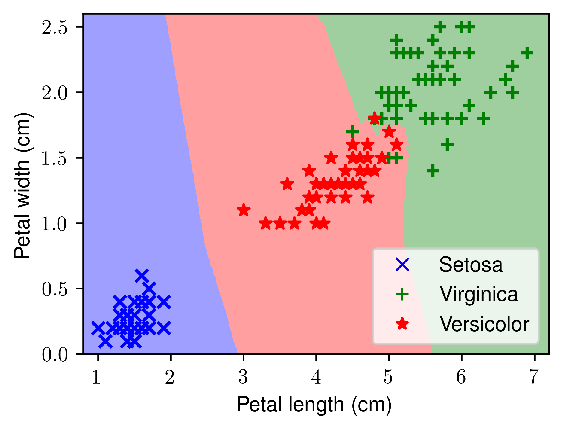
\includegraphics[width=\fourinarow]{figures/classif/knn.pdf}\label{fig:knn}
	}
	\subfloat[\cart{}.]{
		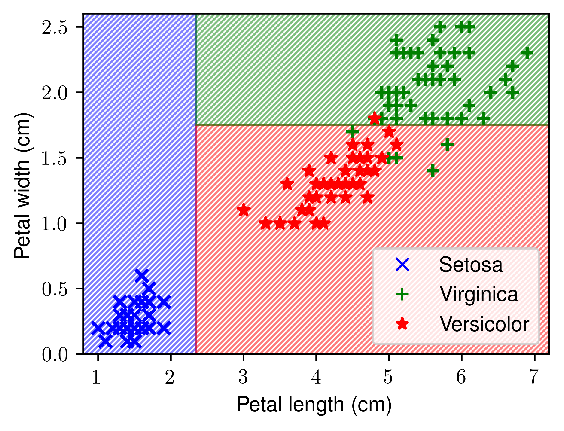
\includegraphics[width=\fourinarow]{figures/classif/cart.pdf}\label{fig:cart}
	}
	\subfloat[\iter{}.]{
		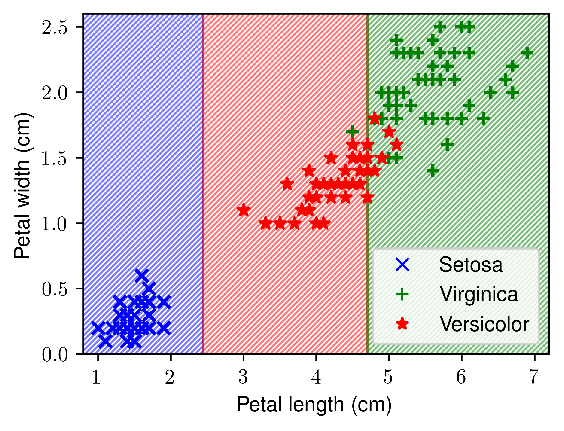
\includegraphics[width=\fourinarow]{figures/classif/iter.pdf}\label{fig:iter}
	}
	\subfloat[\creepy{} (2 features).]{
		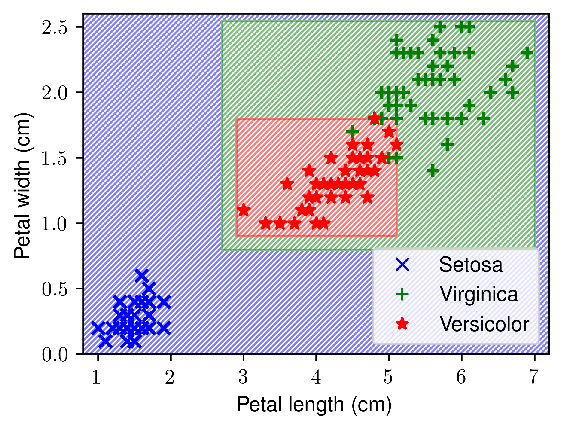
\includegraphics[width=\fourinarow]{figures/classif/creepy2.pdf}\label{fig:creepy2}
	}
	\\
	\subfloat[\creepy{} (1 feature).]{
		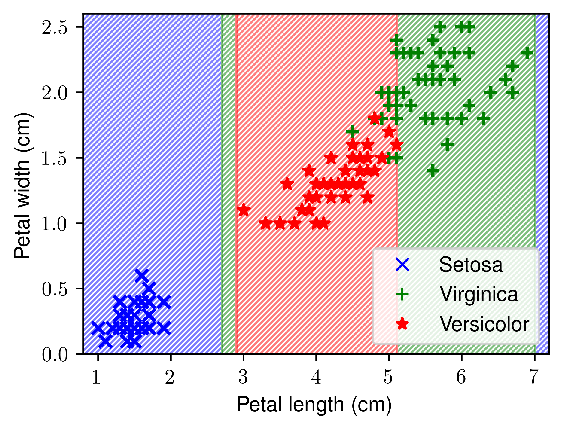
\includegraphics[width=\fourinarow]{figures/classif/creepy1.pdf}\label{fig:creepy1}
	}
	\subfloat[\gridex{} (3 rules).]{
		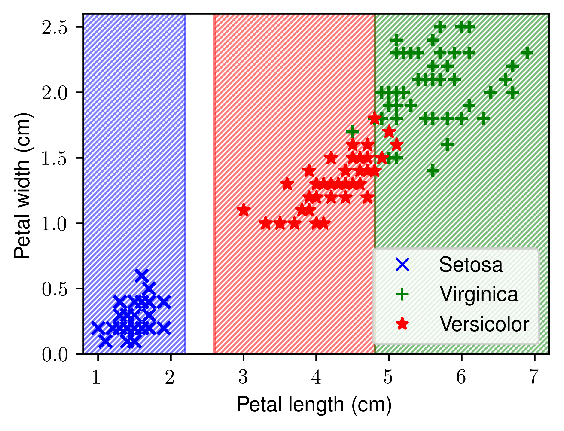
\includegraphics[width=\fourinarow]{figures/classif/gridex3.pdf}\label{fig:gridex3}
	}
	\subfloat[\gridex{} (4 rules).]{
		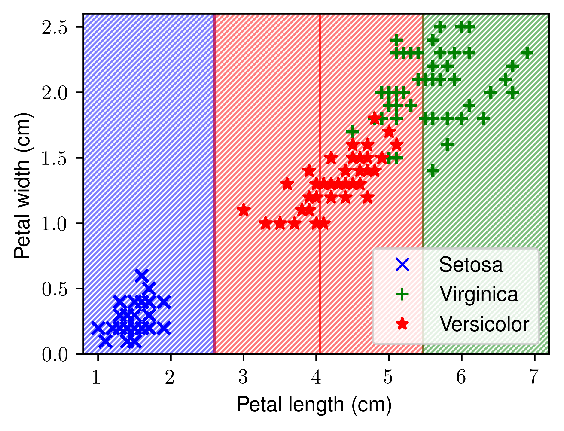
\includegraphics[width=\fourinarow]{figures/classif/gridex4.pdf}\label{fig:gridex4}
	}
	\subfloat[\gridex{} (6 rules).]{
		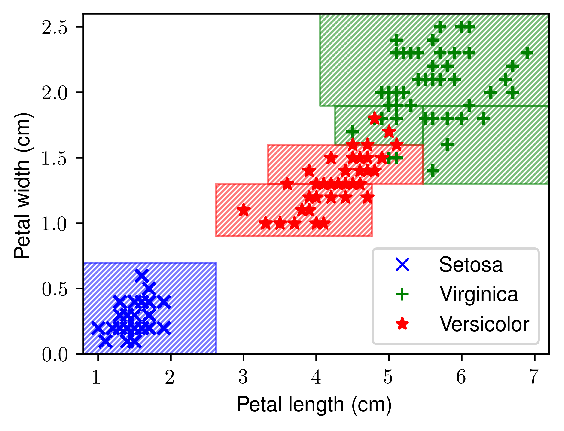
\includegraphics[width=\fourinarow]{figures/classif/gridex6.pdf}\label{fig:gridex6}
	}
	\\
	\subfloat[$Q_s$ quality score.]{
		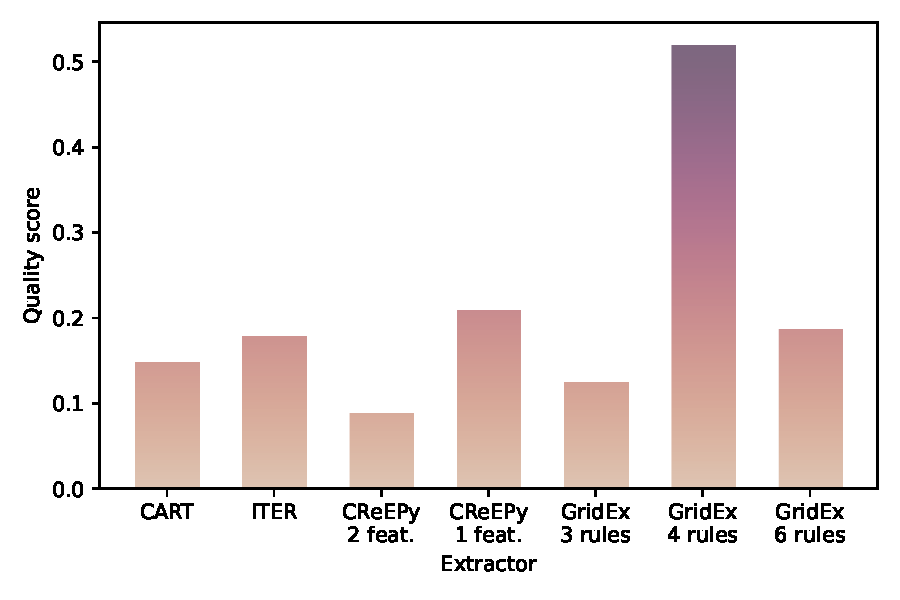
\includegraphics[width=\fourinarow]{figures/qs.pdf}\label{fig:qs}
	}
	\subfloat[$1\textrm{-}\fire{}$.]{
		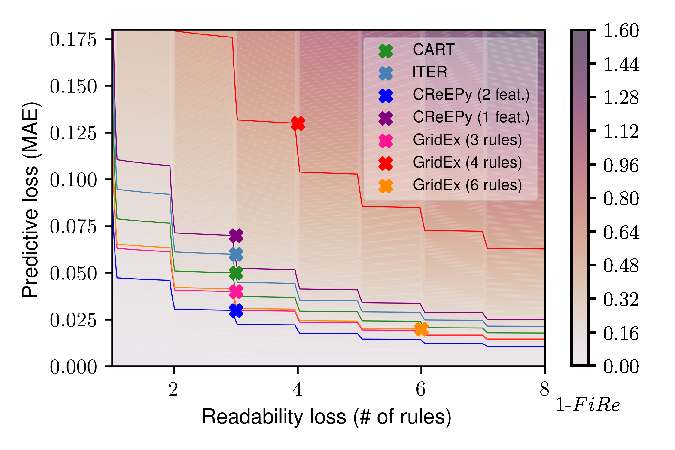
\includegraphics[width=\fourinarow]{figures/exp1.pdf}\label{fig:phi1}
	}
	\subfloat[$2\textrm{-}\fire{}$.]{
		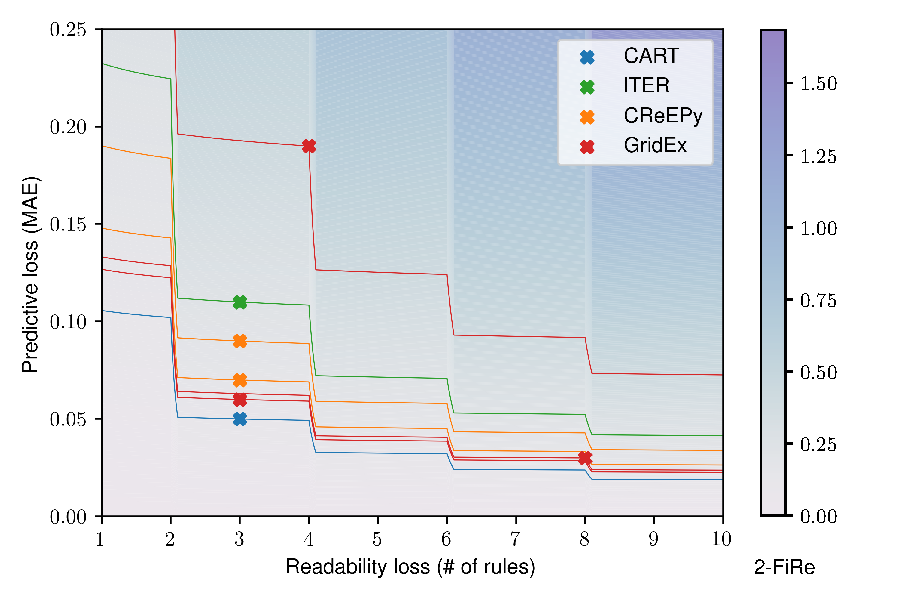
\includegraphics[width=\fourinarow]{figures/exp2.pdf}\label{fig:phi2}
	}
	\subfloat[$3\textrm{-}\fire{}$.]{
		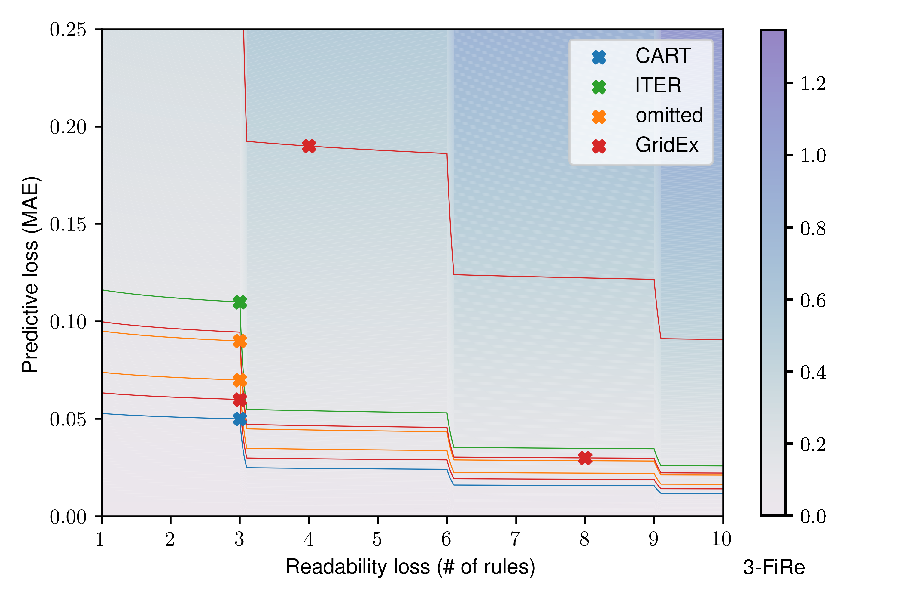
\includegraphics[width=\fourinarow]{figures/exp3.pdf}\label{fig:phi3}
	}
	\caption{Decision boundaries for the Iris data set obtained with different extractors applied to a 9-NN, corresponding quality score $Q_s$ and 1-\fire{}, 2-\fire{} and 3-\fire{} score isolines.}\label{fig:experiments}
\end{figure*}

\begin{table*}[t]\centering
	\begin{tabular}{|c||c|c|c|c|c||c|c|c|c|}
		\toprule
		Algorithm & Accuracy & Coverage & Extracted & Predictive & Coverage & $Q_s$ & \multicolumn{3}{c|}{\psifire{}} \\
		& & & rules ($r$) & loss ($p$) & loss ($c$) & & $\psi=1$ & $\psi=2$ & $\psi=3$ \\
		\midrule\midrule
		9-NN & 0.97 & - & - & - & - & - & - & - & - \\
		\midrule
		\cart{} & 0.95 & 1.00 & 3 & 0.05 & 1.00 & 0.15 & 0.16 & 0.11 & 0.05 \\
		\iter{} & 0.94 & 1.00 & 3 & 0.06 & 1.00 & 0.18 & 0.19 & 0.13 & 0.06 \\
		\creepy{} (2 features) & 0.97 & 1.00 & 3 & 0.03 & 1.00 & \textbf{0.09} & \textbf{0.10} & \textbf{0.06} & \textbf{0.03} \\
		\creepy{} (1 feature) & 0.93 & 1.00 & 3 & 0.07 & 1.00 & 0.21 & 0.22 & 0.15 & 0.07 \\
		\gridex{} (3 rules) & 0.96 & 0.95 & 3 & 0.04 & 1.05 & 0.13 & 0.13 & 0.08 & 0.04 \\
		\gridex{} (4 rules) & 0.87 & 1.00 & 4 & 0.13 & 1.00 & 0.52 & 0.56 & 0.28 & 0.28 \\
		\gridex{} (6 rules) & 0.98 & 0.43 & 6 & 0.02 & 1.57 & 0.19 & 0.13 & 0.07 & 0.04 \\
		\bottomrule
	\end{tabular}
	\caption{Quality assessments for the knowledge extracted by different SKE algorithms from a 9-NN for the Iris data set.}
	\label{tab:experiments}
\end{table*}

Different behaviours can be observed, for instance, by selecting an extracted knowledge composed of a single rule with MAE = 1.5 (green cross).
%
In this case, the scores are evaluated as follows:
%
\begin{equation*}
	2\textrm{-}\fire(1.5, 1)=1.5 < 2.14 = 2\textrm{-}\fire(1.0, 4),
\end{equation*}
%
\begin{equation*}
	6\textrm{-}\fire(1.5, 1)=1.5 > 1.07 = 6\textrm{-}\fire(1.0, 4),
\end{equation*}
%
and their interpretation leads to opposite conclusions.
%
In particular, the single-ruled knowledge is considered better than the others lying on the isoline if considering $\psi=2$.
%
On the other hand, it is worse if considering $\psi=6$.

The dual situation can be encountered with knowledge having 5 rules and MAE = 0.8 (red cross).
%
In this case, the knowledge quality is considered better when evaluated through the 6-\fire{} score and worse with the 2-\fire{} score.

Given all these remarks, we suggest selecting the most adequate value of the $\psi$ parameter for the task after observing the corresponding isolines.

%%%%%%%%%%%%%%%%%%%%%%%
\section{Experiments and discussion}\label{sec:experiments}
%%%%%%%%%%%%%%%%%%%%%%%

The effectiveness of the \fire{} score in evaluating and comparing the quality of SKE techniques' extracted knowledge has been assessed by running several experiments.%\footnote{Code available at \url{https://github.com/psykei/psyke-python/blob/demo/AAAI23/FiRe/demo/DemoFire.ipynb}}
%
In particular, the \psyke{} framework\footnote{Experiments can be reproduced by installing the package from \url{https://github.com/psykei/psyke-python}}~\cite{psyke-woa2021,psyke-extraamas2022,psyke-ia2022} has been used to train a BB predictor and a set of extractors on the well-known Iris dataset\footnote{\url{https://archive.ics.uci.edu/ml/datasets/iris}}~\cite{iris}.
%
The adopted extractors are the following: \cart{}~\cite{breiman1984classification}, \iter{}~\cite{huysmans2006iter}, \creepy{}~\cite{psyke-woa2021} and \gridex{}~\cite{gridex-extraamas2021}.
%
All these techniques have been applied to a $k$-nearest neighbour ($k$-NN) classifier, having $k=9$.
%
Since all the extractors are pedagogical algorithms, the provided output knowledge has been extracted only by observing the input/output response of the 9-NN.
%
We highlight that the choice of a simple data set is only bound to the possibility of easily depicting the decision boundaries given by the models, enabling also a visual comparison of the resulting knowledge.
%
Since the \fire{} score is based on the predictive and readability loss notions, it can be applied to any model for which it is possible to express a predictive loss and a readability loss, regardless of the underlying model and data set complexity and peculiarities, and without any loss of generalisation.

To better understand the example, we recall that \cart{} induces a decision tree classifier on the 9-NN predictions and it has been executed with the default parameters.

On the other hand, \iter{}, \creepy{} and \gridex{} produce a hypercubic partitioning of the input feature space according to different strategies.
%
\iter{} creates and expands cubes in a bottom-up iterative fashion.
%
It relies on 4 hyper-parameters:
%
\begin{inlinelist}
	\item the number of starting cubes, set to 1;
	\item the minimum amount of instances to consider inside each cube, set to 75;
	\item the size of cube updates, set to 7\% of each input feature range interval;
	\item the maximum number of iterations to be performed, set to 600.
\end{inlinelist}

\gridex{} partitions the input feature space in a top-down recursive and symmetric manner, starting from the whole space.
%
It relies on 4 hyper-parameters:
%
\begin{inlinelist}
	\item the maximum depth of the recursive splitting;
	\item the minimum amount of instances to consider inside each cube, set to 1;
	\item the number of slices to perform at each iteration;
	\item the error threshold to decide if a hypercubic region should be further partitioned, set to 0.1.
\end{inlinelist}
%
An error threshold equal to 0.1 means that all cubes having an accuracy smaller than 0.9 are further split.
%
The number of slices to perform has been adaptively chosen.
%
In particular, our experiments, resumed in \Cref{tab:experiments}, consider 3 \gridex{} instances.
%
The first and the second perform 8 and 2 slices, respectively, only along the most relevant input feature.
%
The third performs 4 slices on the 2 most relevant input dimensions.
%
As for the maximum depth, the first instance has a value equal to 1, and the others equal to 2.

\creepy{} adopts an underlying clustering technique to divide the input space into hypercubic hierarchical regions.
%
We set equal to 2 the maximum depth parameter and equal to 0.1 the error threshold, which has the same semantics as that of \gridex{}.
%
For our experiments, we trained 2 \creepy{} instances, one considering the most relevant input feature and the other considering also the second one.

The classification accuracy of each extractor, as well as that of the 9-NN, has been reported in \Cref{tab:experiments}.
%
The table also shows the number of extracted rules, representing the readability loss $r$ of the extractors.
%
Analogously, the predictive loss $p$ is reported as $1-accuracy$.
%
The coverage achieved by the extraction techniques is reported as the portion of input space covered by the corresponding knowledge, in percentage.
%
The coverage loss has been calculated as $2-coverage$, according to the definition by~\citet{skemetrics-aaai2023}.
%
Finally, the last four columns report the quality scores associated with each extractor.
%
Best scores are highlighted with bold font.
%
We compared the \psifire{} scores calculated for different values of $\psi$ with the quality score ($Q_s$) described by~\citet{skemetrics-aaai2023}.
%
Data has been averaged upon 5 executions for each extractor.
%
The results' standard deviation has been omitted since each algorithm provided very similar outputs at every execution.

Graphical representations of the decision boundaries given by the 9-NN and the extractors are reported in \Cref{fig:experiments}.
%
The bottom row of the figure reports the quality assessments.
%
In particular, the $Q_s$ score is reported in \Cref{fig:qs}, whereas \Cref{fig:phi1,fig:phi2,fig:phi3} show the isolines for the \psifire{} scores adopted in the experiments.
%
It is important to focus on the fact that it is not possible to obtain less than 3 rules, since the Iris data set describes 3 output classes and in the best case extracted knowledge contains a rule per distinct class.

From \Cref{tab:experiments} and \Cref{fig:experiments} it is evident that \creepy{} considering 2 input features is the SKE algorithm providing the best output knowledge in terms of coverage, readability and predictive performance.
%
Indeed, it has the lowest $Q_s$ and \psifire{} scores regardless of the adopted $\psi$.
%
This result is true and acceptable since \creepy{} is the algorithm providing the smallest amount of rules with the smallest predictive error.

Different conclusions may be drawn by comparing \cart{}, the \gridex{} instance providing a knowledge with 3 rules and the one providing 6 rules according to different quality scores.
%
Indeed, according to the $Q_s$ score, the best knowledge amongst these is the one having 3 rules and obtained via \gridex{} ($Q_s=0.13$), whereas the \gridex{} instance providing 6 rules is the worst choice ($Q_s=0.19$).
%
\cart{}'s quality is assessed with $Q_s=0.15$, representing a middle evaluation between the two \gridex{} instances.
%
\gridex{} providing 6 rules is considered as the worst algorithm despite its minimum predictive loss since it has very high readability and coverage losses w.r.t.\ \cart{} and the other \gridex{} instance.
%
\cart{} is considered slightly worse than \gridex{} providing 3 rules despite having the same readability loss because \gridex{} has a higher coverage loss that is more than compensated by a better predictive loss.

The comparison amongst the same three algorithms performed via the \fire{} scores leads to different conclusions.
%
In particular, the \fire{} score neglects the coverage loss and the quality is assessed only based on the predictive and readability losses.
%
For this reason the two \gridex{} instances are considered always better than \cart{}, regardless of the chosen $\psi$ value, since \cart{} has a higher predictive loss that is not compensated by its small readability loss.
%
The $\psi$ parameter, however, affects the comparison between the two \gridex{} instances, that are evaluated with the same quality score with $\psi=1$ and $\psi=3$.
%
Only in these cases the fluctuations in the predictive and readability losses are compensated by the user-defined fidelity/readability trade-off value.

%%%%%%%%%%%%%%%%%%%%%%%
\section{Conclusions}\label{sec:conclusions}
%%%%%%%%%%%%%%%%%%%%%%%

In this paper we present \fire{}, a scoring function to evaluate and compare SKE algorithms.
%
More precisely, it is a compact score encompassing both a readability assessment and a predictive performance evaluation and it may be exploited to help users choose the best extraction procedure w.r.t.\ a specific fidelity/readability trade-off, expressed as a parameter.
%
The \fire{} score may also be applied together with automatic parameter-tuning procedures.
%
We show here the properties of the scoring function and a rigorous mathematical formulation is also provided.

Our future works will focus on enhancing the \fire{} score concerning its readability loss parameter, with a more expressive formulation than the mere amount of rules provided as output by an extractor.

\section*{Acknowledgments}

This work has been partially supported by the EU ICT-48 2020 project TAILOR (No. 952215).

%%%%%%%%%%%%%%%%%%%%%%%%
%\section*{Ethics statement}
%%%%%%%%%%%%%%%%%%%%%%%%
%The authors confirm that proper consideration has been given to any ethics issues. The data sets considered for the experiments do not contain any sensitive features and were treated in compliance with all existing data laws. Being related to the explainability of decisions made by AI systems, the work can have a substantial impact on ethics, ensuring greater transparency and traceability of the decisions made, and guaranteeing equitable and fair approaches. Therefore it could contribute to building more trustable and therefore more ethical systems.

%% The file named.bst is a bibliography style file for BibTeX 0.99c
\bibliographystyle{kr}
\bibliography{fire-ijcai-23}

\end{document}

